\chapter{Results \& Conclusion}
\label{chap:conclusion}
\setlength{\parskip}{1.5mm}
%\setlength{\baselineskip}{1.4mm}

The entire top level module was simulated in Xilinx Vivado and the synthesis and working of each of the modules were verified. The functions of encryption \& decryption modules were also analysed. The results obtained in the hardware simulation matches with the state variable values simulated in MATLAB within some reasonable accuracy.

\begin{figure}[H]
\centering
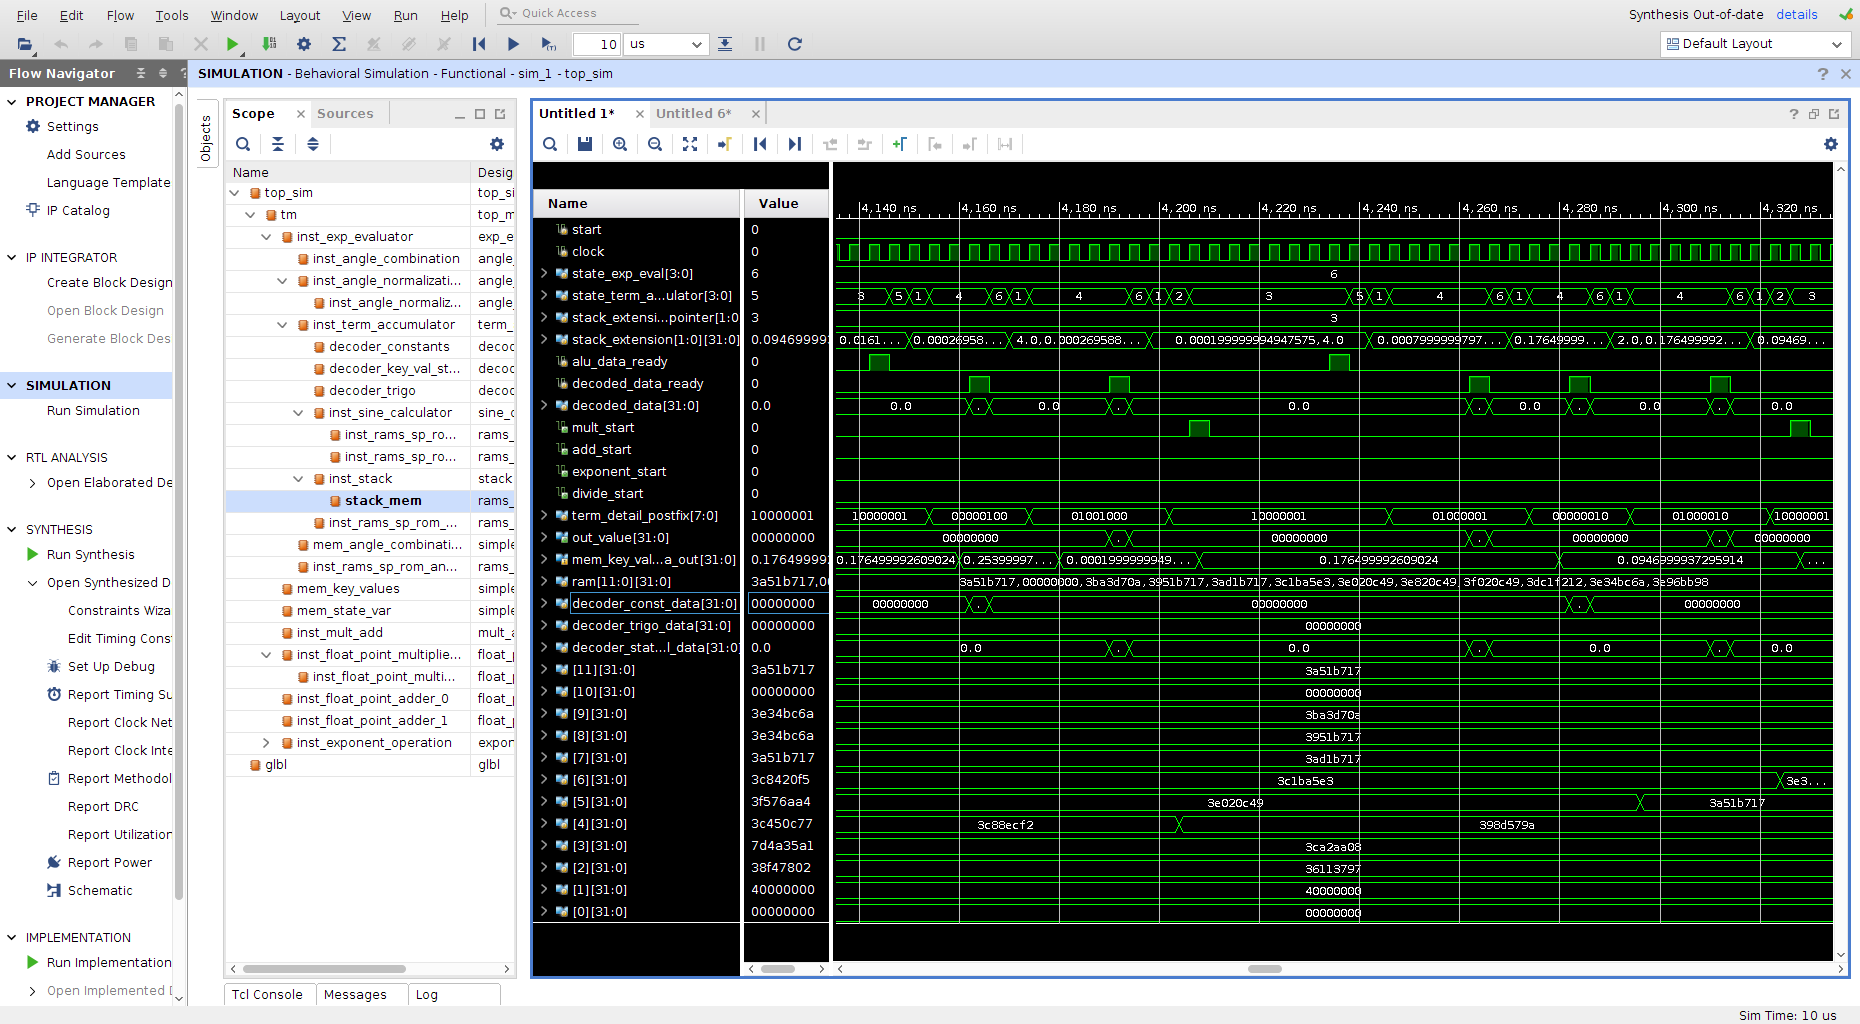
\includegraphics[width=16cm]{vivado_simulation.png}
\caption{Simulation of hardware implementation  in Xilinx Vivado}\label{fig:vivado_simulation}
\end{figure}

From the analysis presented in section 5.5 and the results obtained from the hardware simulation of the FPGA implementation, we can conclude that this design can serve as a good prototype of a chaos based cryptographic hardware which is immune against brute force quantum computing attacks.
